\section{Constrained rigid body dynamics\label{constraints}}

This section is based on material in~\cite{BaraffWitkin:97} and~\cite{Saunders:PhD}. The
explanation in these sources is rather sketchy though, and the following details I worked
out are more comprehensive.

\subsection{Prerequisites of constraint solving\label{constraintPrerequisites}}

Consider a system of $n$ rigid bodies at a particular point in time. Assume that we can define
a vector \ve{x} which represents the state of the whole system as a function of
time\footnote{Witkin~\cite{BaraffWitkin:97} calls this vector \ve{q}; I use \ve{x} to avoid
confusion with quaternions.}. \ve{x} has $6n$ rows (one row for each d.o.f.)\ and its first and
second derivative with respect to time are
\begin{equation}
\label{lagrangeStateVector}
\dot{\ve{x}} = \left[ \begin{array}{c}
    \dot{\ve{r}}_1\\ \ve{\omega}_1\\ \vdots\\ \dot{\ve{r}}_n\\ \ve{\omega}_n \end{array}\right]
\quad\quad\mathrm{and}\quad\quad
\ddot{\ve{x}} = \left[ \begin{array}{c}
    \ddot{\ve{r}}_1\\ \dot{\ve{\omega}}_1\\ \vdots\\ \ddot{\ve{r}}_n\\ \dot{\ve{\omega}}_n
    \end{array}\right]
\end{equation}
where $\ve{r}_i$ is the position of the centre of mass of body $i$, and $\ve{\omega}_i$ is its
angular velocity. Thus $\dot{\ve{x}}$ is the concatenation of all bodies' linear and angular
velocities, and $\ddot{\ve{x}}$ is that of the accelerations. We cannot write down an explicit
expression for \ve{x} since we do not have a representation of orientation whose derivative is
\ve{\omega}. This is not a problem though, since we can work exclusively with $\dot{\ve{x}}$ and
$\ddot{\ve{x}}$.

We require two more vectors in the same format, containing the forces and torques already acting
on the system, for example due to gravity or muscular activity:
\begin{equation} \label{PhiVector}
\ve{\Phi} = \left[\begin{array}{c}
    \ve{F}_1 \\ \ve{\tau}_1 \\ \vdots \\ \ve{F}_n \\ \ve{\tau}_n
    \end{array}\right]
    \quad\quad\quad
\ve{\Phi}_p = \left[\begin{array}{c}
    \ve{0} \\ -\dual{\ve{\omega}_1}\m{I}_1\ve{\omega}_1 \\ \vdots \\
    \ve{0} \\ -\dual{\ve{\omega}_n}\m{I}_n\ve{\omega}_n
    \end{array}\right]
\end{equation}

Here $\ve{F}_i$ denotes the sum of all forces acting on the centre of mass of body~$i$, and
$\ve{\tau}_i$ is the sum of all torque vectors acting on body~$i$. The vector $\ve{\Phi}_p$
accounts for the fact that a body's moment of inertia is in general not constant in the world
frame\footnote{The subscript $p$ of this vector stands for \emph{precession}, since the
variability of the moment of inertia causes free precession.}; $\m{I}_i$ is body $i$'s moment
of inertia in the world frame at the current point in time.
See appendix~\ref{correctBrettAppendix} for a derivation of $\ve{\Phi}_p$.

Following the same principle of concatenation, we set up the inverse mass-inertia matrix
$\m{M}^{-1}$, a $6n\times6n$ matrix of the form
\begin{equation}
\label{massInertiaTensor}
\m{M}^{-1} = \left[ \begin{array}{ccccccc}
    \frac{1}{\mu_1}\m{1} \\ & \m{I}_1^{-1} \\ &&
    \frac{1}{\mu_2}\m{1} \\ &&& \m{I}_2^{-1} \\ &&&& \ddots \\ &&&&&
    \frac{1}{\mu_n}\m{1} \\ &&&&&& \m{I}_n^{-1}
    \end{array}\right]
\end{equation}

$\mu_i$ denotes the (scalar) mass of body $i$, \m{1} stands for the $3\times3$
identity matrix, and $\m{I}_i^{-1}$ is the inverse of the inertia tensor (written as a
$3\times3$ matrix) of body $i$ in the world frame. All empty regions are zero. While $\mu_i$
will typically stay constant over time, $\m{I}_i$ may depend on the orientation of body
$i$.\footnote{If we know the principal axes of the body, we can express \m{I} in a time-invariant
form combined with rotations into the principal axes frame and back again
(see~\cite{BaraffWitkin:97}), which saves us a lot of effort.} These variables have been chosen
such that
\begin{equation}
\ddot{\ve{x}} = \m{M}^{-1} (\ve{\Phi} + \ve{\Phi}_p).
\end{equation}


\subsection{Definition of the Jacobians\label{jacDefinition}}

Now assume that we want to impose $m$ constraints on this system. Express each constraint as a function
$c$ which is zero when the constraint is satisfied.  We can then concatenate all
constraint functions into a single $m$-row constraint vector \ve{c}. Each valid configuration of
the system must satisfy $\ve{c} = \ve{0}$. $\dot{\ve{c}}$ and $\ddot{\ve{c}}$ must be calculated
algebraically before implementation.

The Jacobian matrix~\cite{RHB:02} \m{J} contains all partial derivatives of $\ve{c}$ w.r.t.\ each
coordinate of \ve{x}. Similarly, $\dot{\m{J}}$ is the Jacobian of $\dot{\ve{c}}$:
\begin{equation}
J_{ij} = \frac{\partial c_i}{\partial x_j} \quad\quad\mathrm{and}\quad\quad
\dot{J}_{ij} = \frac{\partial \dot{c}_i}{\partial x_j}
\end{equation}

Both $\m{J}$ and $\dot{\m{J}}$ are $m \times 6n$ matrices. However, since we do not
have an explicit expression for \ve{x}, we cannot calculate them directly using
partial differentiation. Instead we make use of the following analytic results:
\begin{equation}
\label{cDotAndCDDot}
\dot{\ve{c}} = \m{J}\dot{\ve{x}} \quad\quad\mathrm{and}\quad\quad
\ddot{\ve{c}} = \dot{\m{J}}\dot{\ve{x}} + \m{J}\ddot{\ve{x}}.
\end{equation}

Any Jacobian component $J_{ij}$ is certainly zero if constraint $i$ does not mention body
$\lfloor j/6 \rfloor$. Since each constraints usually involves only two bodies, \m{J} and
$\dot{\m{J}}$ each have a sparse block-structured form sketched in figure~\ref{jacobianFigure}.
If there are many constraints, their slices of the Jacobian can be calculated independently and
simply inserted at the right places in \m{J} and $\dot{\m{J}}$. Appendix~\ref{constraintAppendix}
gives derivations of Jacobian slices for different constraint types.

\begin{figure}
\psfrag{frag:1}{$1$}
\psfrag{frag:i}{$i$}
\psfrag{frag:j}{$j$}
\psfrag{frag:m}{$m$}
\psfrag{frag:6n}{$6n$}
\psfrag{frag:jac}{$\m{J}=\left(\rule{54mm}{0mm}\rule{0mm}{20mm}\right)$}
\psfrag{frag:b1}{$\begin{array}{c} b_1 \\ \overbrace{\rule{0mm}{5mm}} \end{array}$}
\psfrag{frag:b2}{$\begin{array}{c} b_2 \\ \overbrace{\rule{0mm}{5mm}} \end{array}$}
\psfrag{frag:ci}{$\ve{c}_i$}
\centerline{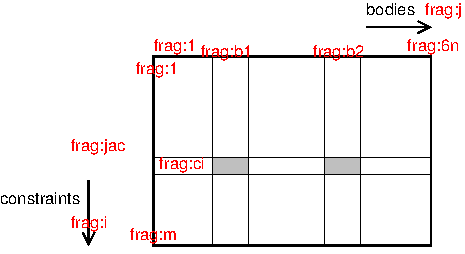
\includegraphics{figures/jacobian}}
\caption[]{Block structure of the Jacobian matrix of $m$ constraints in a system of $n$ bodies.
    For example, if $\ve{c}_i$ is a ball-and-socket joint between bodies $b_1$ and $b_2$, each of
    the two slices (shaded areas) is three rows high and six columns wide. The vertical position
    of $\ve{c}_i$ must match its offset in the concatenated constraint vector \hbox{\ve{c}}, and
    the horizontal positions of the slices must match the offset of bodies $b_1$ and $b_2$ in the
    vectors $\dot{\ve{x}}$, \ve{\Phi} and $\ve{\Phi}_p$ (equations~\ref{lagrangeStateVector}
    and~\ref{PhiVector}). \label{jacobianFigure}}
\end{figure}


\subsection{Finding the Jacobians\label{jacCalculation}}

Both~\cite{BaraffWitkin:97} and~\cite{Saunders:PhD} omit details on how to derive the Jacobians
$\m{J}$ and $\dot{\m{J}}$ for a custom constraint. I deduced the following procedure
after pondering over some source code implementing one type of constraint
(specifically equations~\ref{constrEx1J} and~\ref{constrEx1JDot} below). The source code
was kindly provided by Dr.~Breton Saunders~\cite{Saunders}. It was used only for this
derivation and not copied otherwise. The implementation in this project is based on the
following derivations.

We start by defining a function $\ve{c}$ which evaluates to zero (or the null vector) for
all states which satisfy the constraint, and any non-zero value for all other states.
We then calculate the first and second derivatives with respect to time, $\dot{\ve{c}}$
and $\ddot{\ve{c}}$, which must both exist.

For any sort of valid constraint, we should be able to massage both $\dot{\ve{c}}$ and
$\ddot{\ve{c}}$ into a sum of products form. Moreover, in each summand in
$\dot{\ve{c}}$, at least one of the variables should be either the linear velocity of
the centre of mass of one of the bodies, or the angular velocity of one of the bodies.
Use algebra to make this `chosen variable' the rightmost variable in each product, and
evaluate the rest of the product to a single matrix.

Now observe equation~\ref{cDotAndCDDot} (page~\pageref{cDotAndCDDot}). We can easily
factor our expression for
$\dot{\ve{c}}$ into $\m{J}$ and $\dot{\ve{x}}$ (since the latter contains
the linear and angular velocities for all bodies). $\m{J}$ has the same number of rows
as there are constraints, and $6n$ columns for a system of $n$ bodies. Each of the matrices
in our expression for $\dot{\ve{c}}$ also has the same number of rows as there are
constraints, and has 3 columns. All we need to do is to find the correct horizontal position
of each of these matrices in $\m{J}$, depending on the location of the `chosen variable'
in $\dot{\ve{x}}$. Thus we obtain the matrix $\m{J}$.

Observe equation~\ref{cDotAndCDDot} again. Now we know $\ddot{\ve{c}}$, $\dot{\ve{x}}$,
$\m{J}$ and $\ddot{\ve{x}}$~-- no problem. Evaluate
$\ddot{\ve{c}} - \m{J}\ddot{\ve{x}}$, remembering that $\ddot{\ve{x}}$ is
the vector of linear accelerations and angular accelerations. The result should be an
expression which we can bring into just the same kind of sum of products form as we previously
did with $\dot{\ve{c}}$. By exactly the same procedure we factor out the linear velocities
and angular velocities (not accelerations!), thus obtaining $\dot{\m{J}}$.

In case you were in doubt, this procedure is of course executed by a human on paper
(possibly assisted by a symbolic algebra system) prior to
implementation. The simulation program will just plug numbers into the hard-coded expressions
for $\ve{c}$, $\dot{\ve{c}}$, $\m{J}$ and $\dot{\m{J}}$ during each time step
of the simulation.
